\subsection{Pagina di un team}
%link all'articolo:
% http://www.f1world.it/team-e-piloti-f1/scuderia-ferrari-f1-2016/
Verrà analizzata una pagina relativa a una squadra del campionato di Formula1.

\begin{figure}[H] % 'h' not 'H'
  \centering
  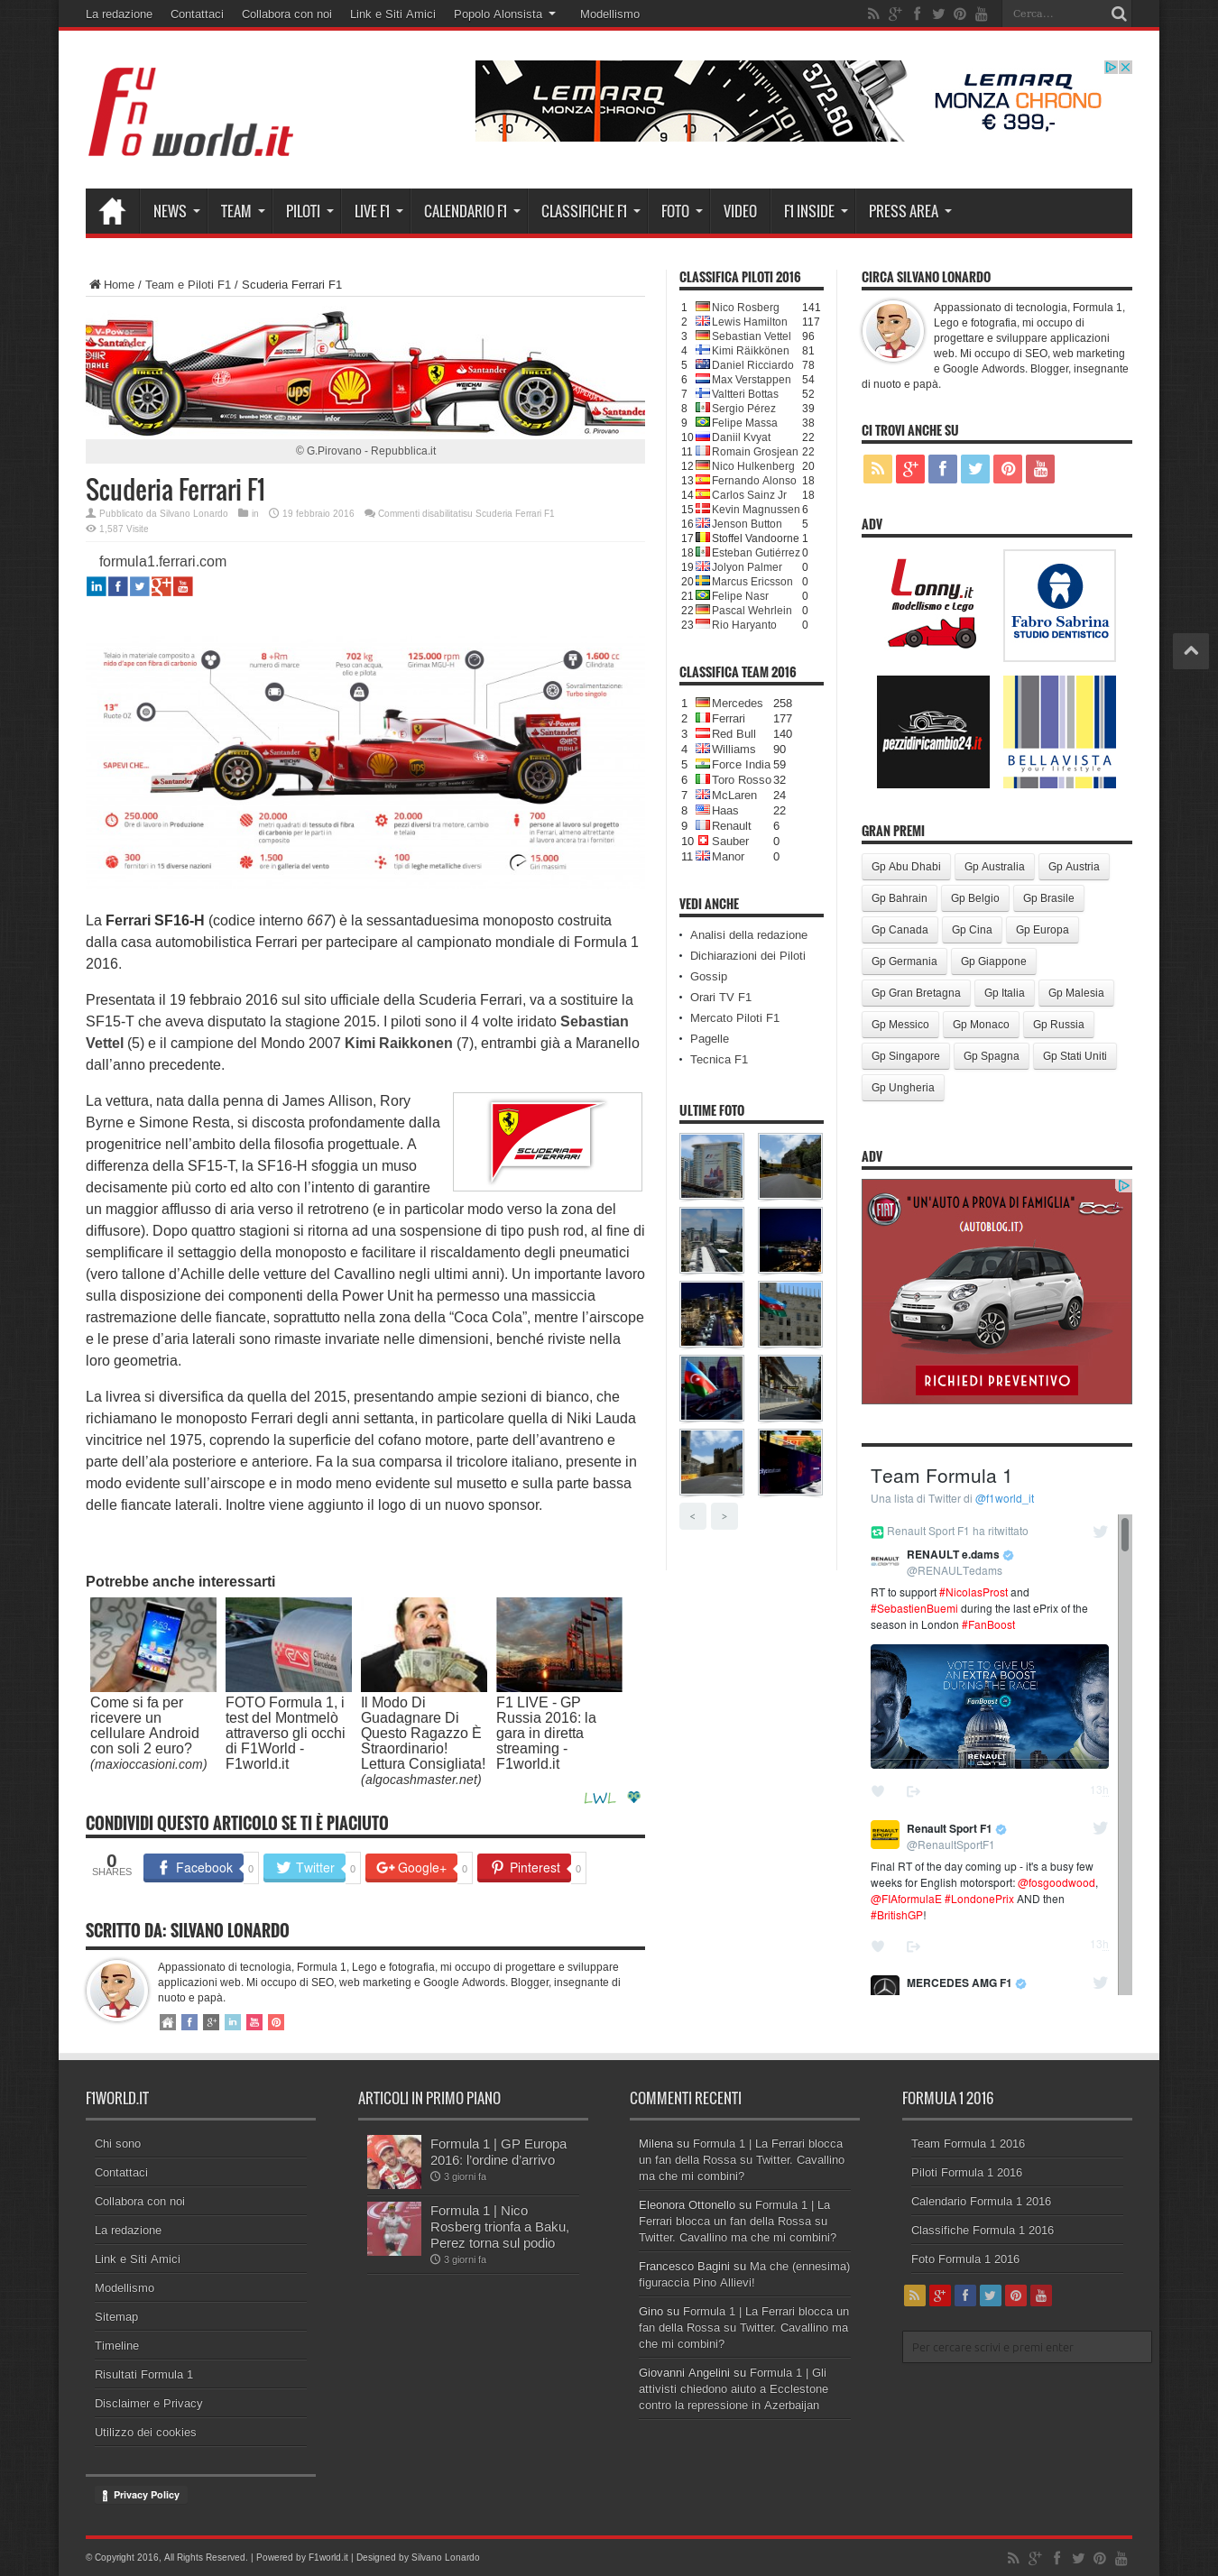
\includegraphics[height=18cm, width=10cm]{res/img/TeamPage_Full}
  \caption{\textit{Screenshot} di una descrizione di una squadra di Formula1}
\end{figure}

È possibile notare come ancora una volta venga messa in risalto l'immagine
rispetto al testo: addirittura prima del titolo della squadra è presente
l'immagine della macchina del campionato corrente. Questa immagine, viene poi
ripetuta dopo il titolo (con maggiori dettagli). Questo secondo me non è un buon
approccio in quanto viene utilizzato spazio utile per poter inserire del testo,
forzando quindi l'utente ad eseguire degli scroll per poter arrivare alle
informazioni desiderate.

Dopo il titolo è presente l'indirizzo \textit{URL} della squadra, seguito dalle
icone per le pagine presenti nei vari social network.

Le informazioni testuali sono ben distribuite: ogni paragrafo, infatti, è
ben distanziato, permettendo all'utente una migliore leggibilità.

Al termine del contenuto, è presente la sezione degli articoli relativi, che
come già descritto presenta al suo interno delle inserzioni pubblicitarie, che
risultano ben integrate dal punto di vista del tema del sito, ma non dal punto
di vista dei contenuti.

È possibile poi condividere la storia della squadra sui più blasonati social
network e infine troviamo le informazioni sull'autore. Queste informazioni
sono ripetute sia alla fine della pagina, sia in alto a destra. Questa
ripetizione risulta superflua e dovrebbe essere eliminata.
